\documentclass[main]{subfiles}


\title[AutoML: Introduction]{AutoML Motivation}
\subtitle{Interfaces to AutoML}
\author[Marius Lindauer]{Marius Lindauer}
\date{}

\titlebackground*{images/AutoML_HPO_2_2}

%\institute{}
%\date{}

\begin{document}
	
	\maketitle
	

%----------------------------------------------------------------------
%----------------------------------------------------------------------
\begin{frame}[c]{Views on AutoML}

\begin{enumerate}

    \item What are the interfaces to AutoML tools? (previous videos)
    \item Which tasks are addressed by AutoML?
    \item Which approaches are being used by AutoML tools?
    \item What can be done in post-processing?
\end{enumerate}

\end{frame}
%-----------------------------------------------------------------------
%----------------------------------------------------------------------
\begin{frame}[c]{Overview AutoML Fields: General}

\centering
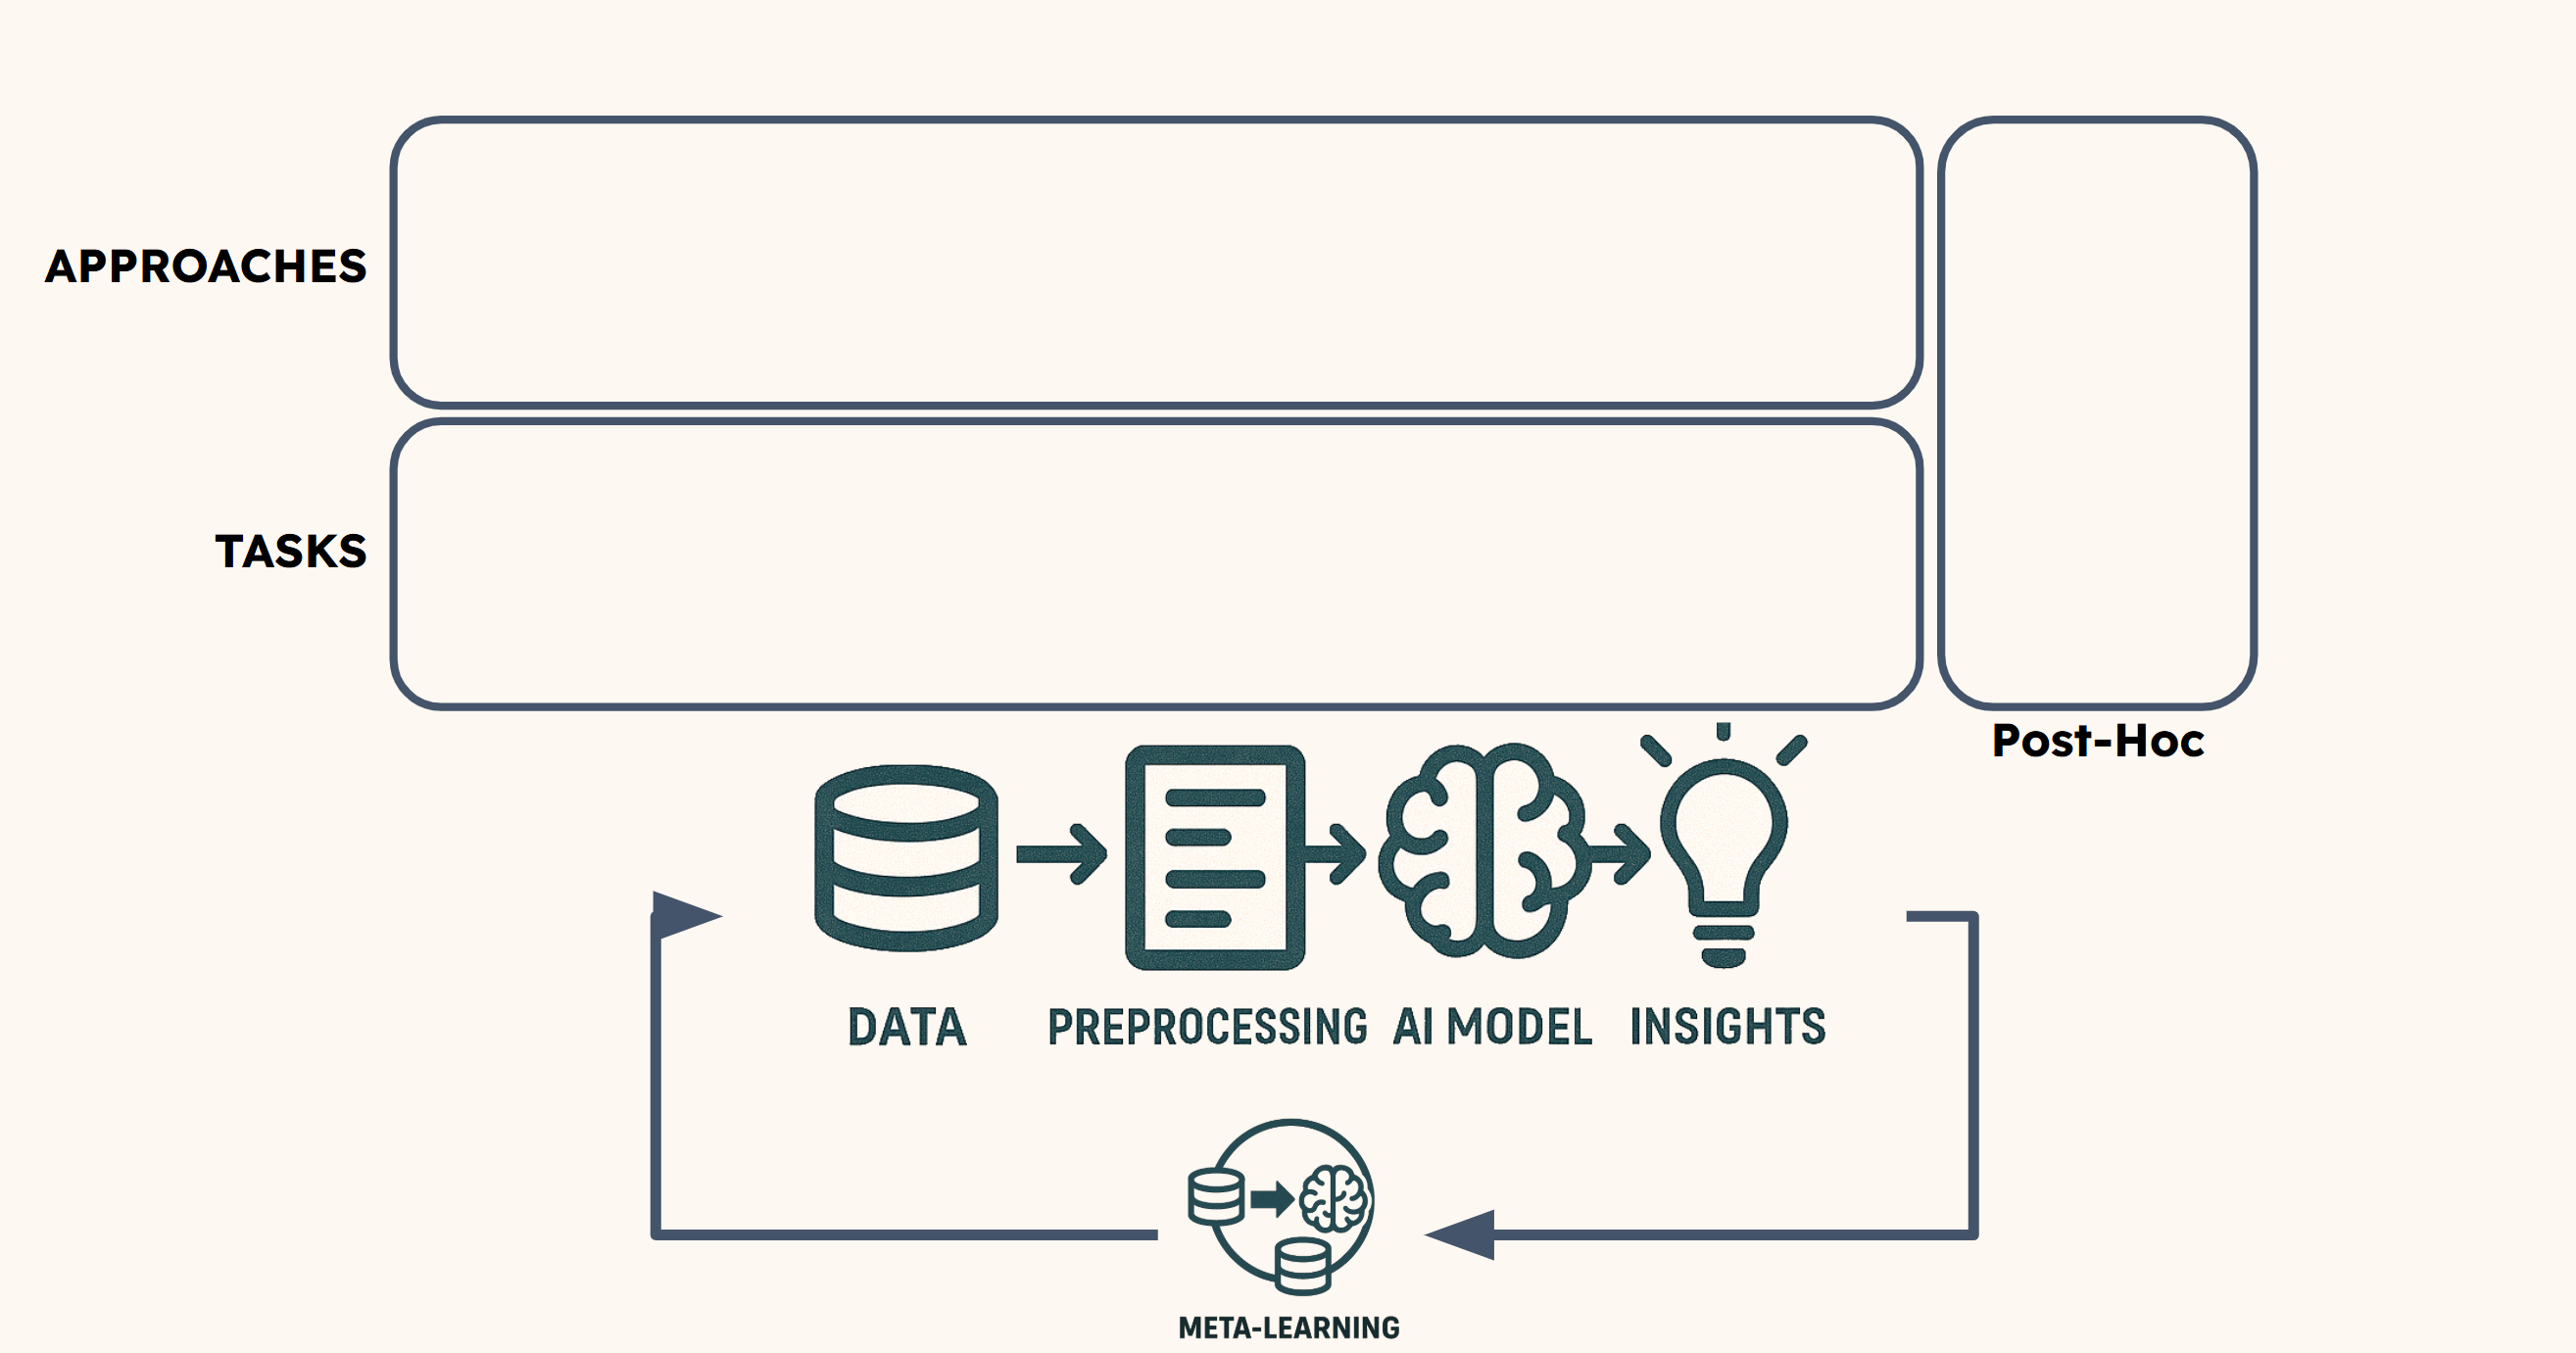
\includegraphics[width=0.8\textwidth]{images/automl_empty.png}


\end{frame}
%-----------------------------------------------------------------------
%----------------------------------------------------------------------
\begin{frame}[c]{Overview AutoML Fields: Tasks}

\centering
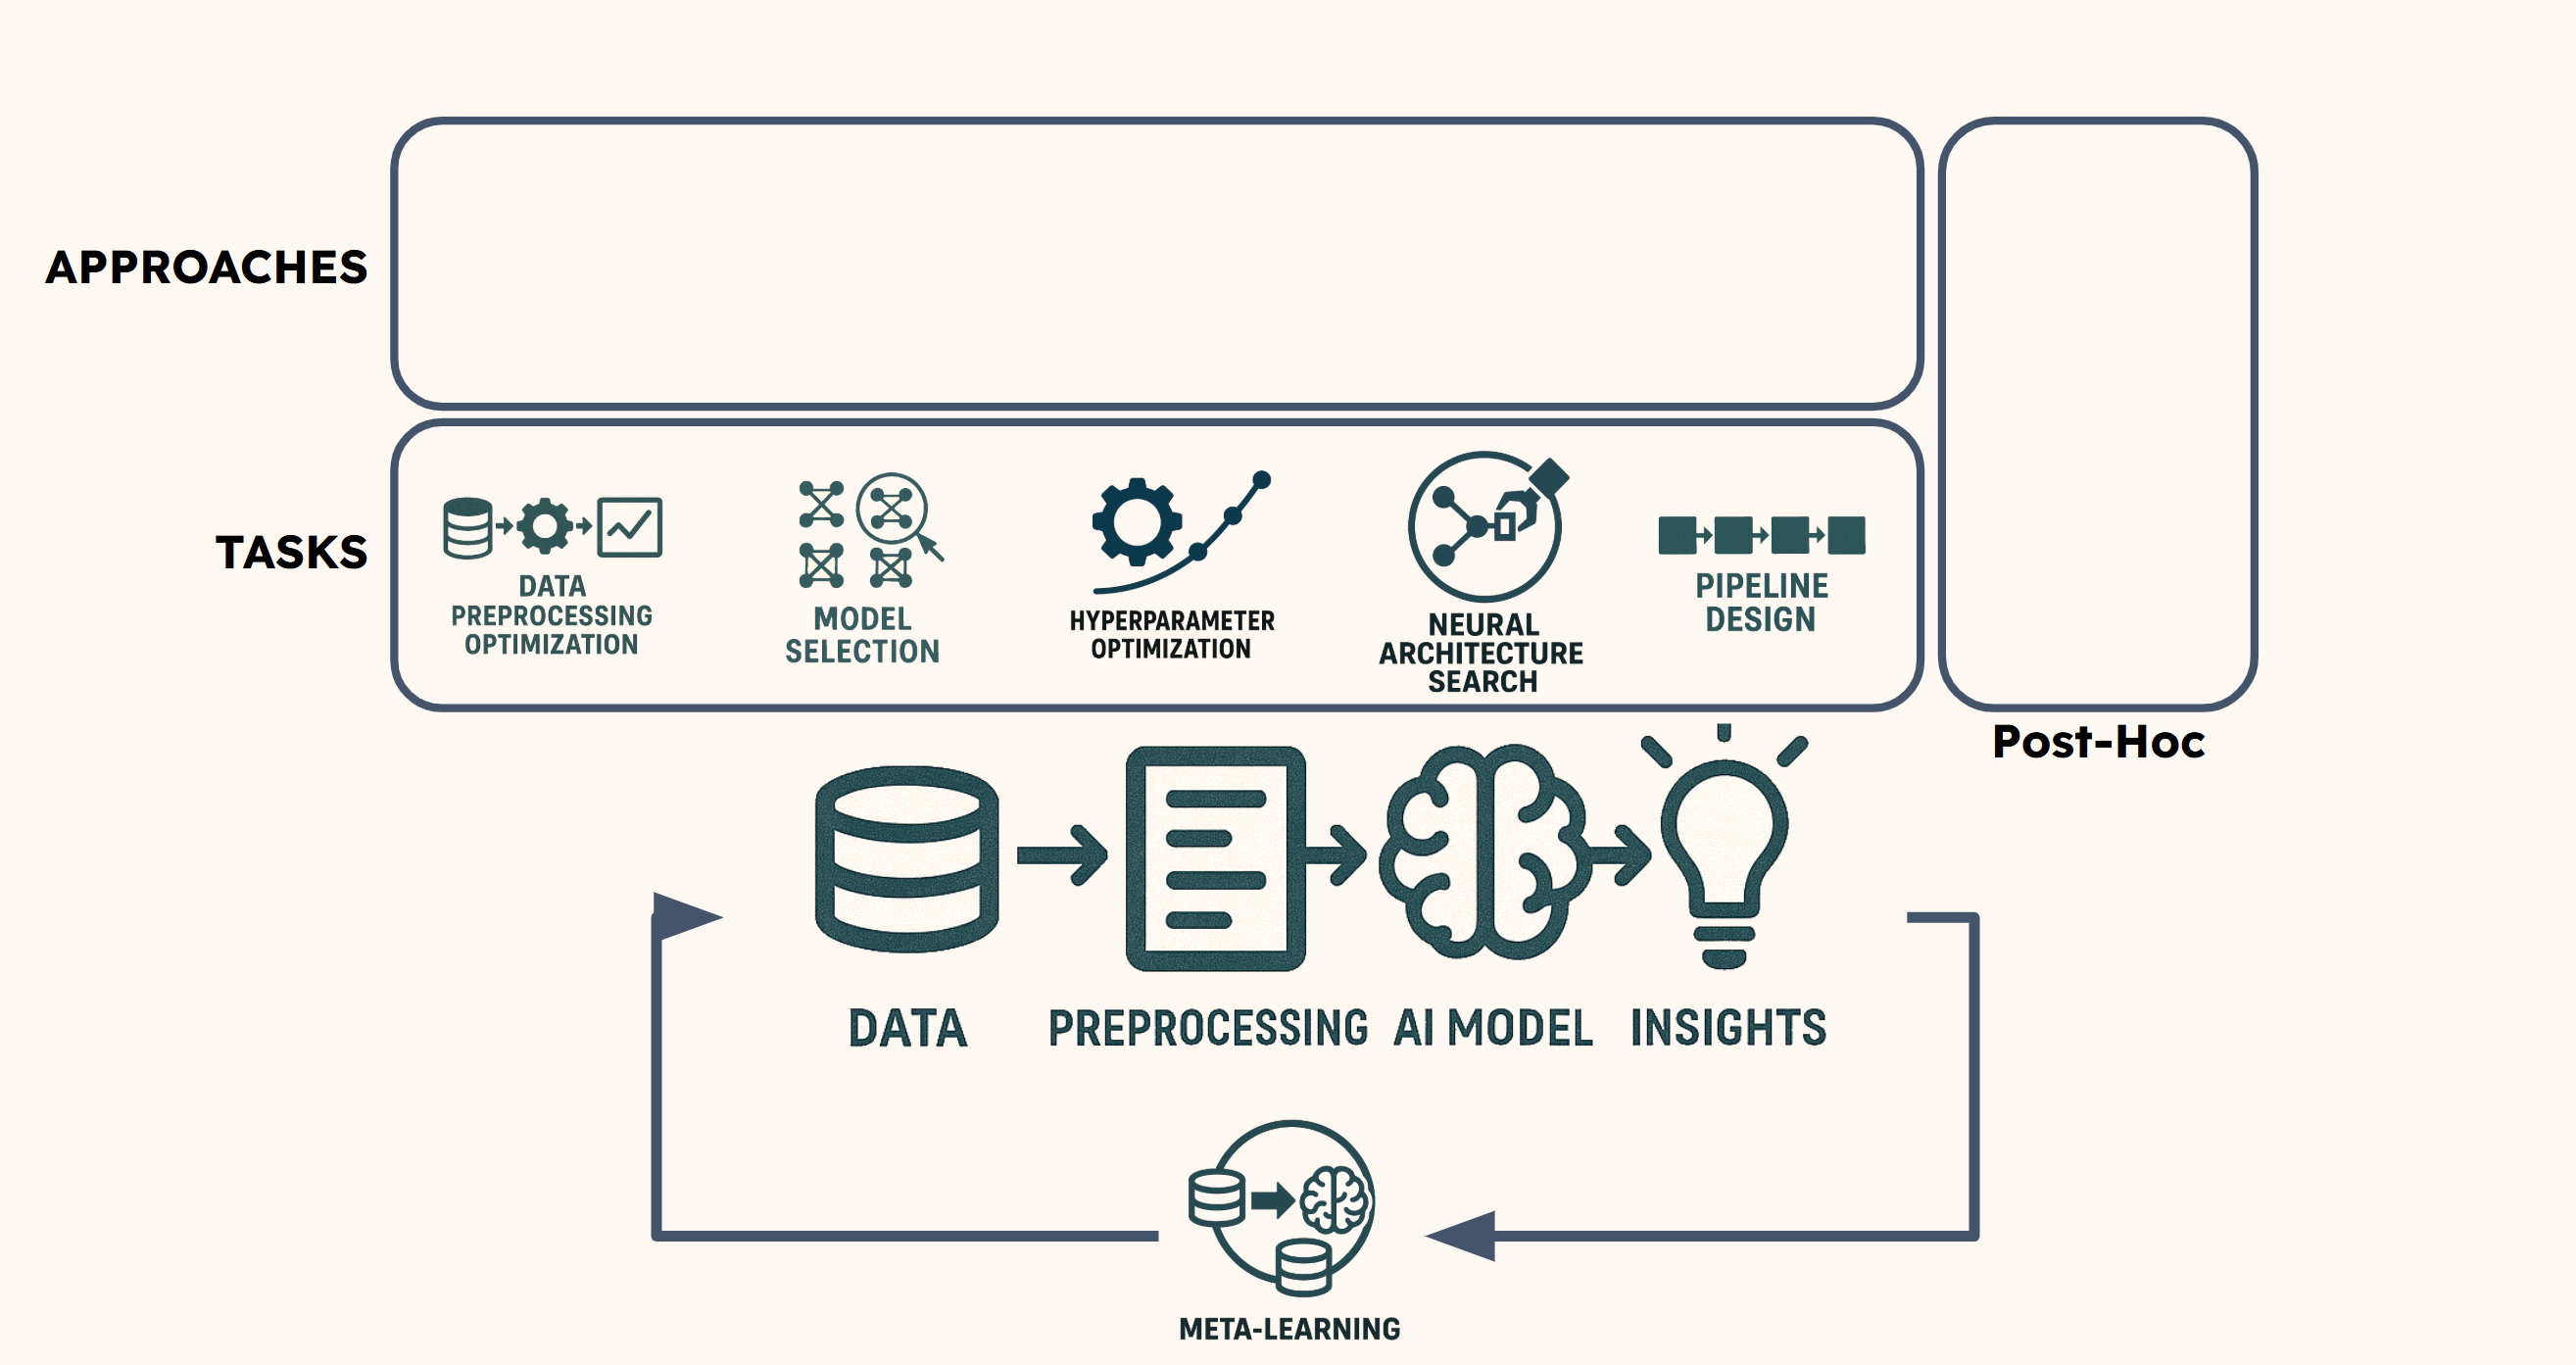
\includegraphics[width=0.8\textwidth]{images/automl_tasks.png}


\end{frame}
%-----------------------------------------------------------------------
%----------------------------------------------------------------------
\begin{frame}[c]{Overview AutoML Fields: Approaches}

\centering
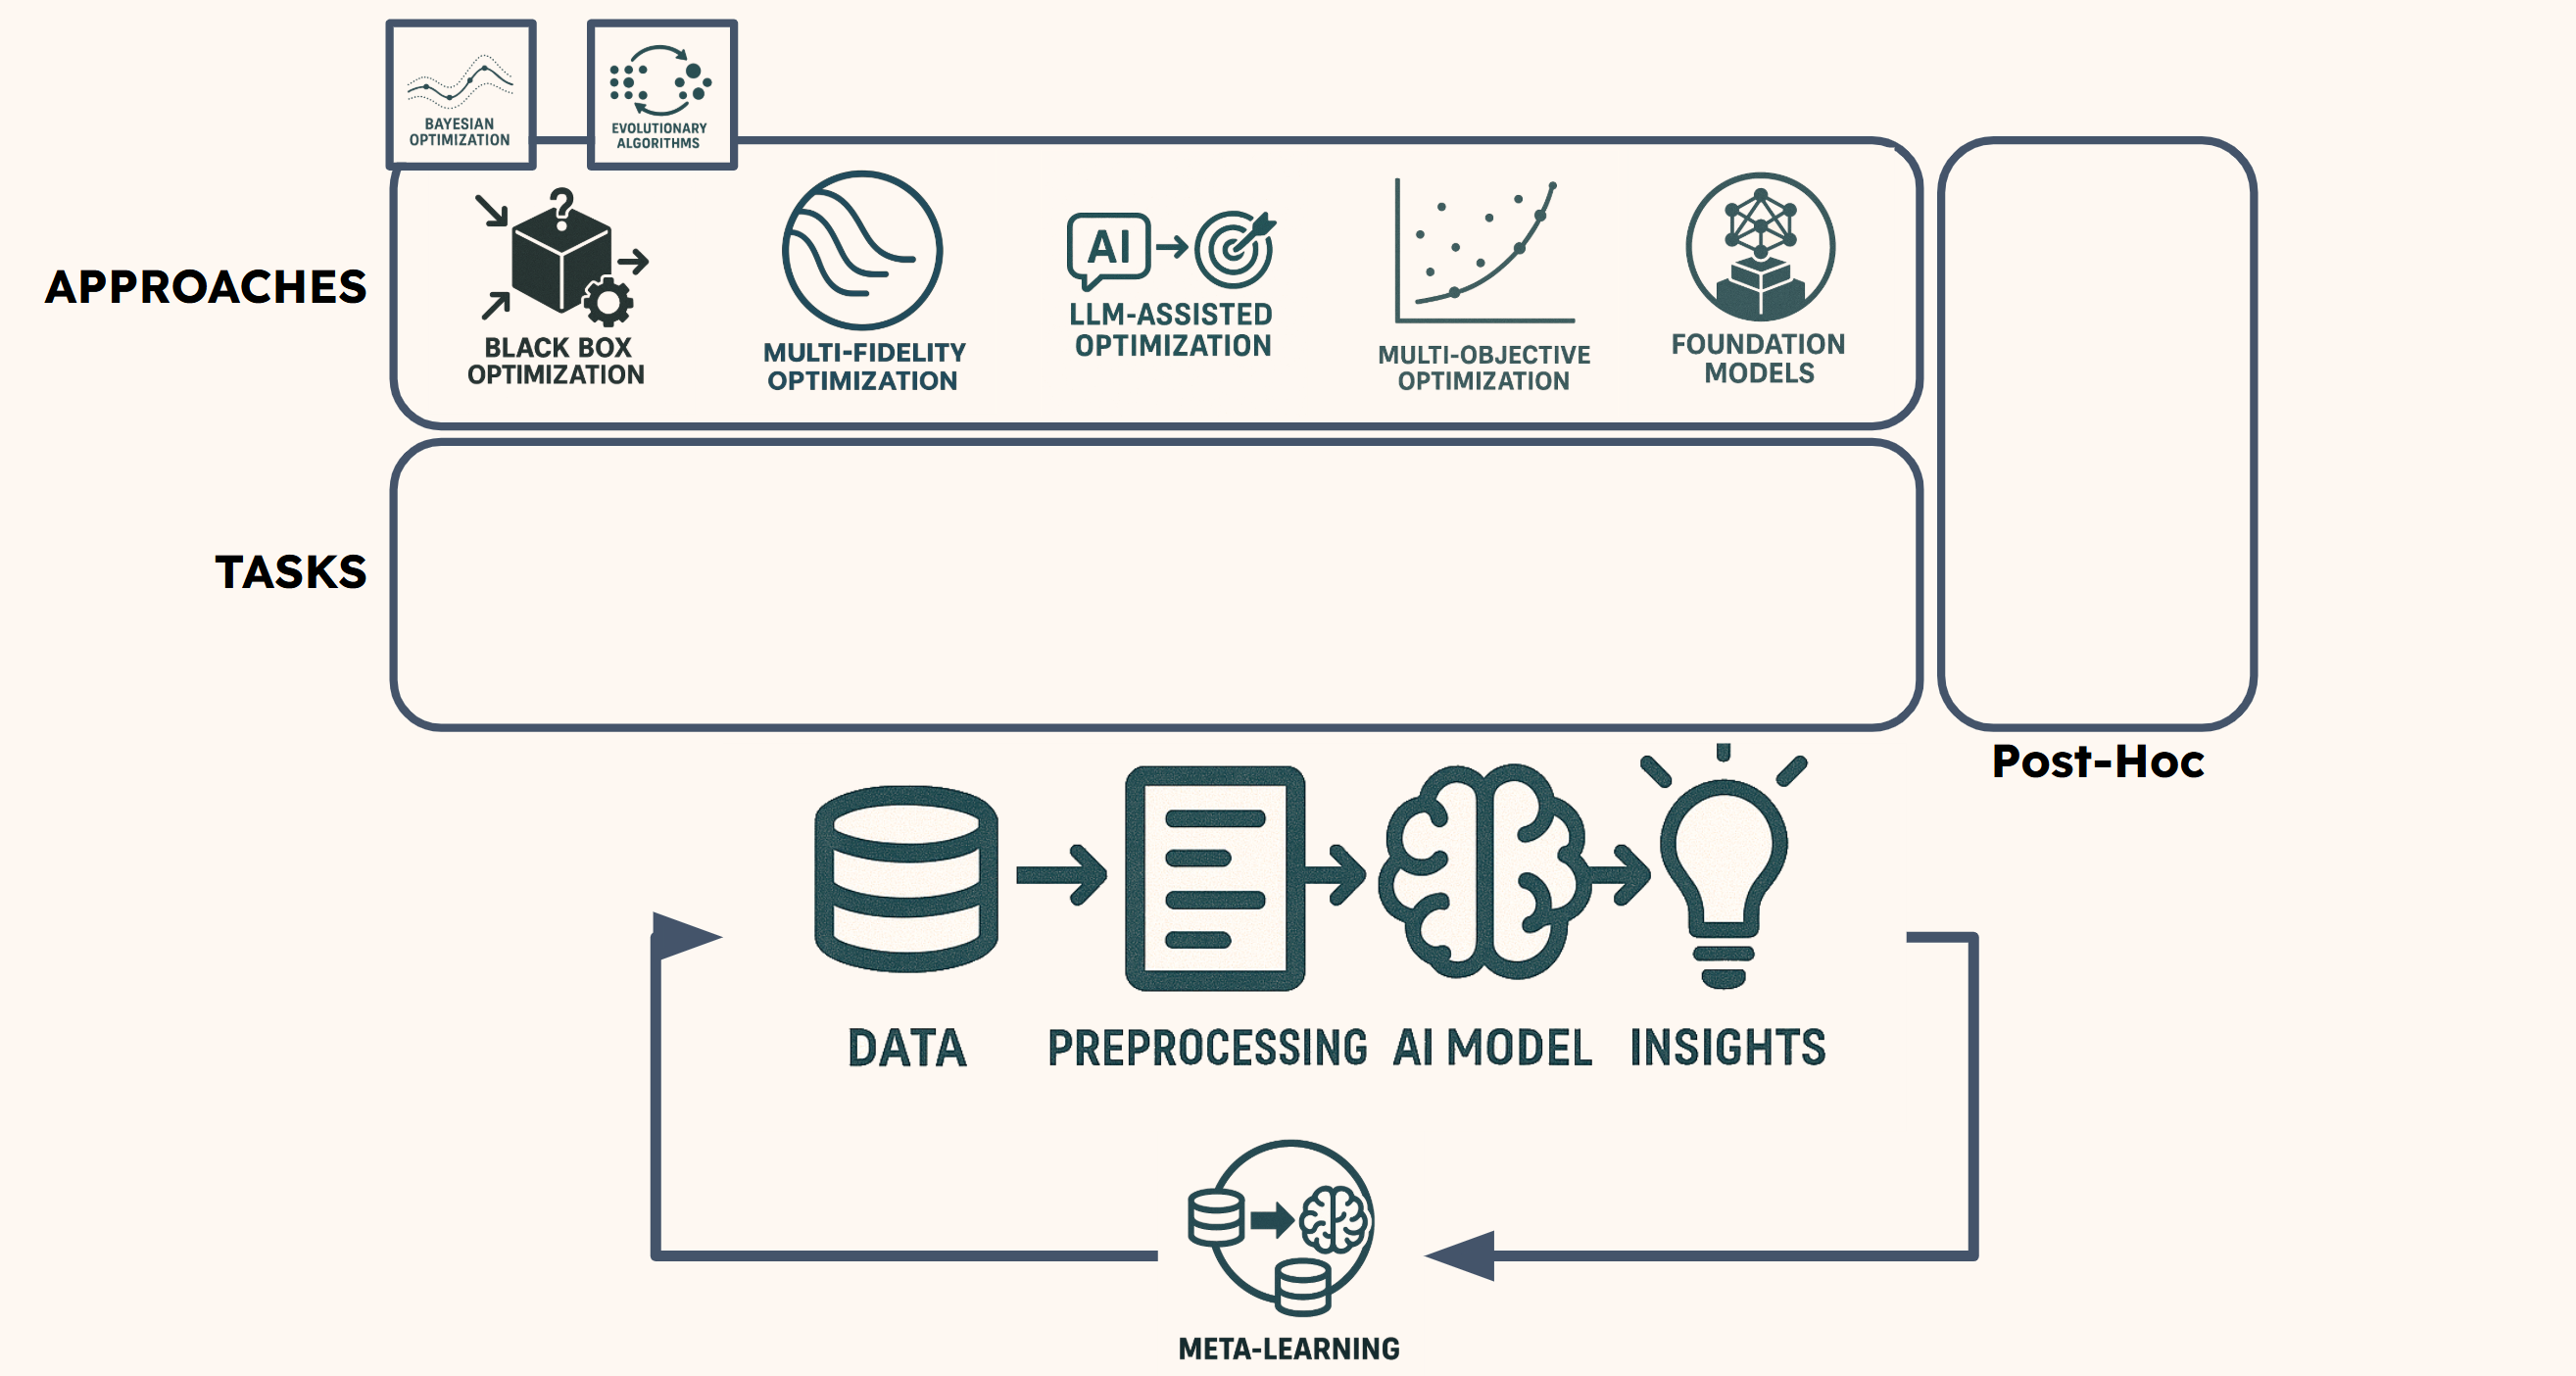
\includegraphics[width=0.8\textwidth]{images/automl_approaches.png}


\end{frame}
%-----------------------------------------------------------------------
%----------------------------------------------------------------------
\begin{frame}[c]{Overview AutoML Fields: Post-hoc}

\centering
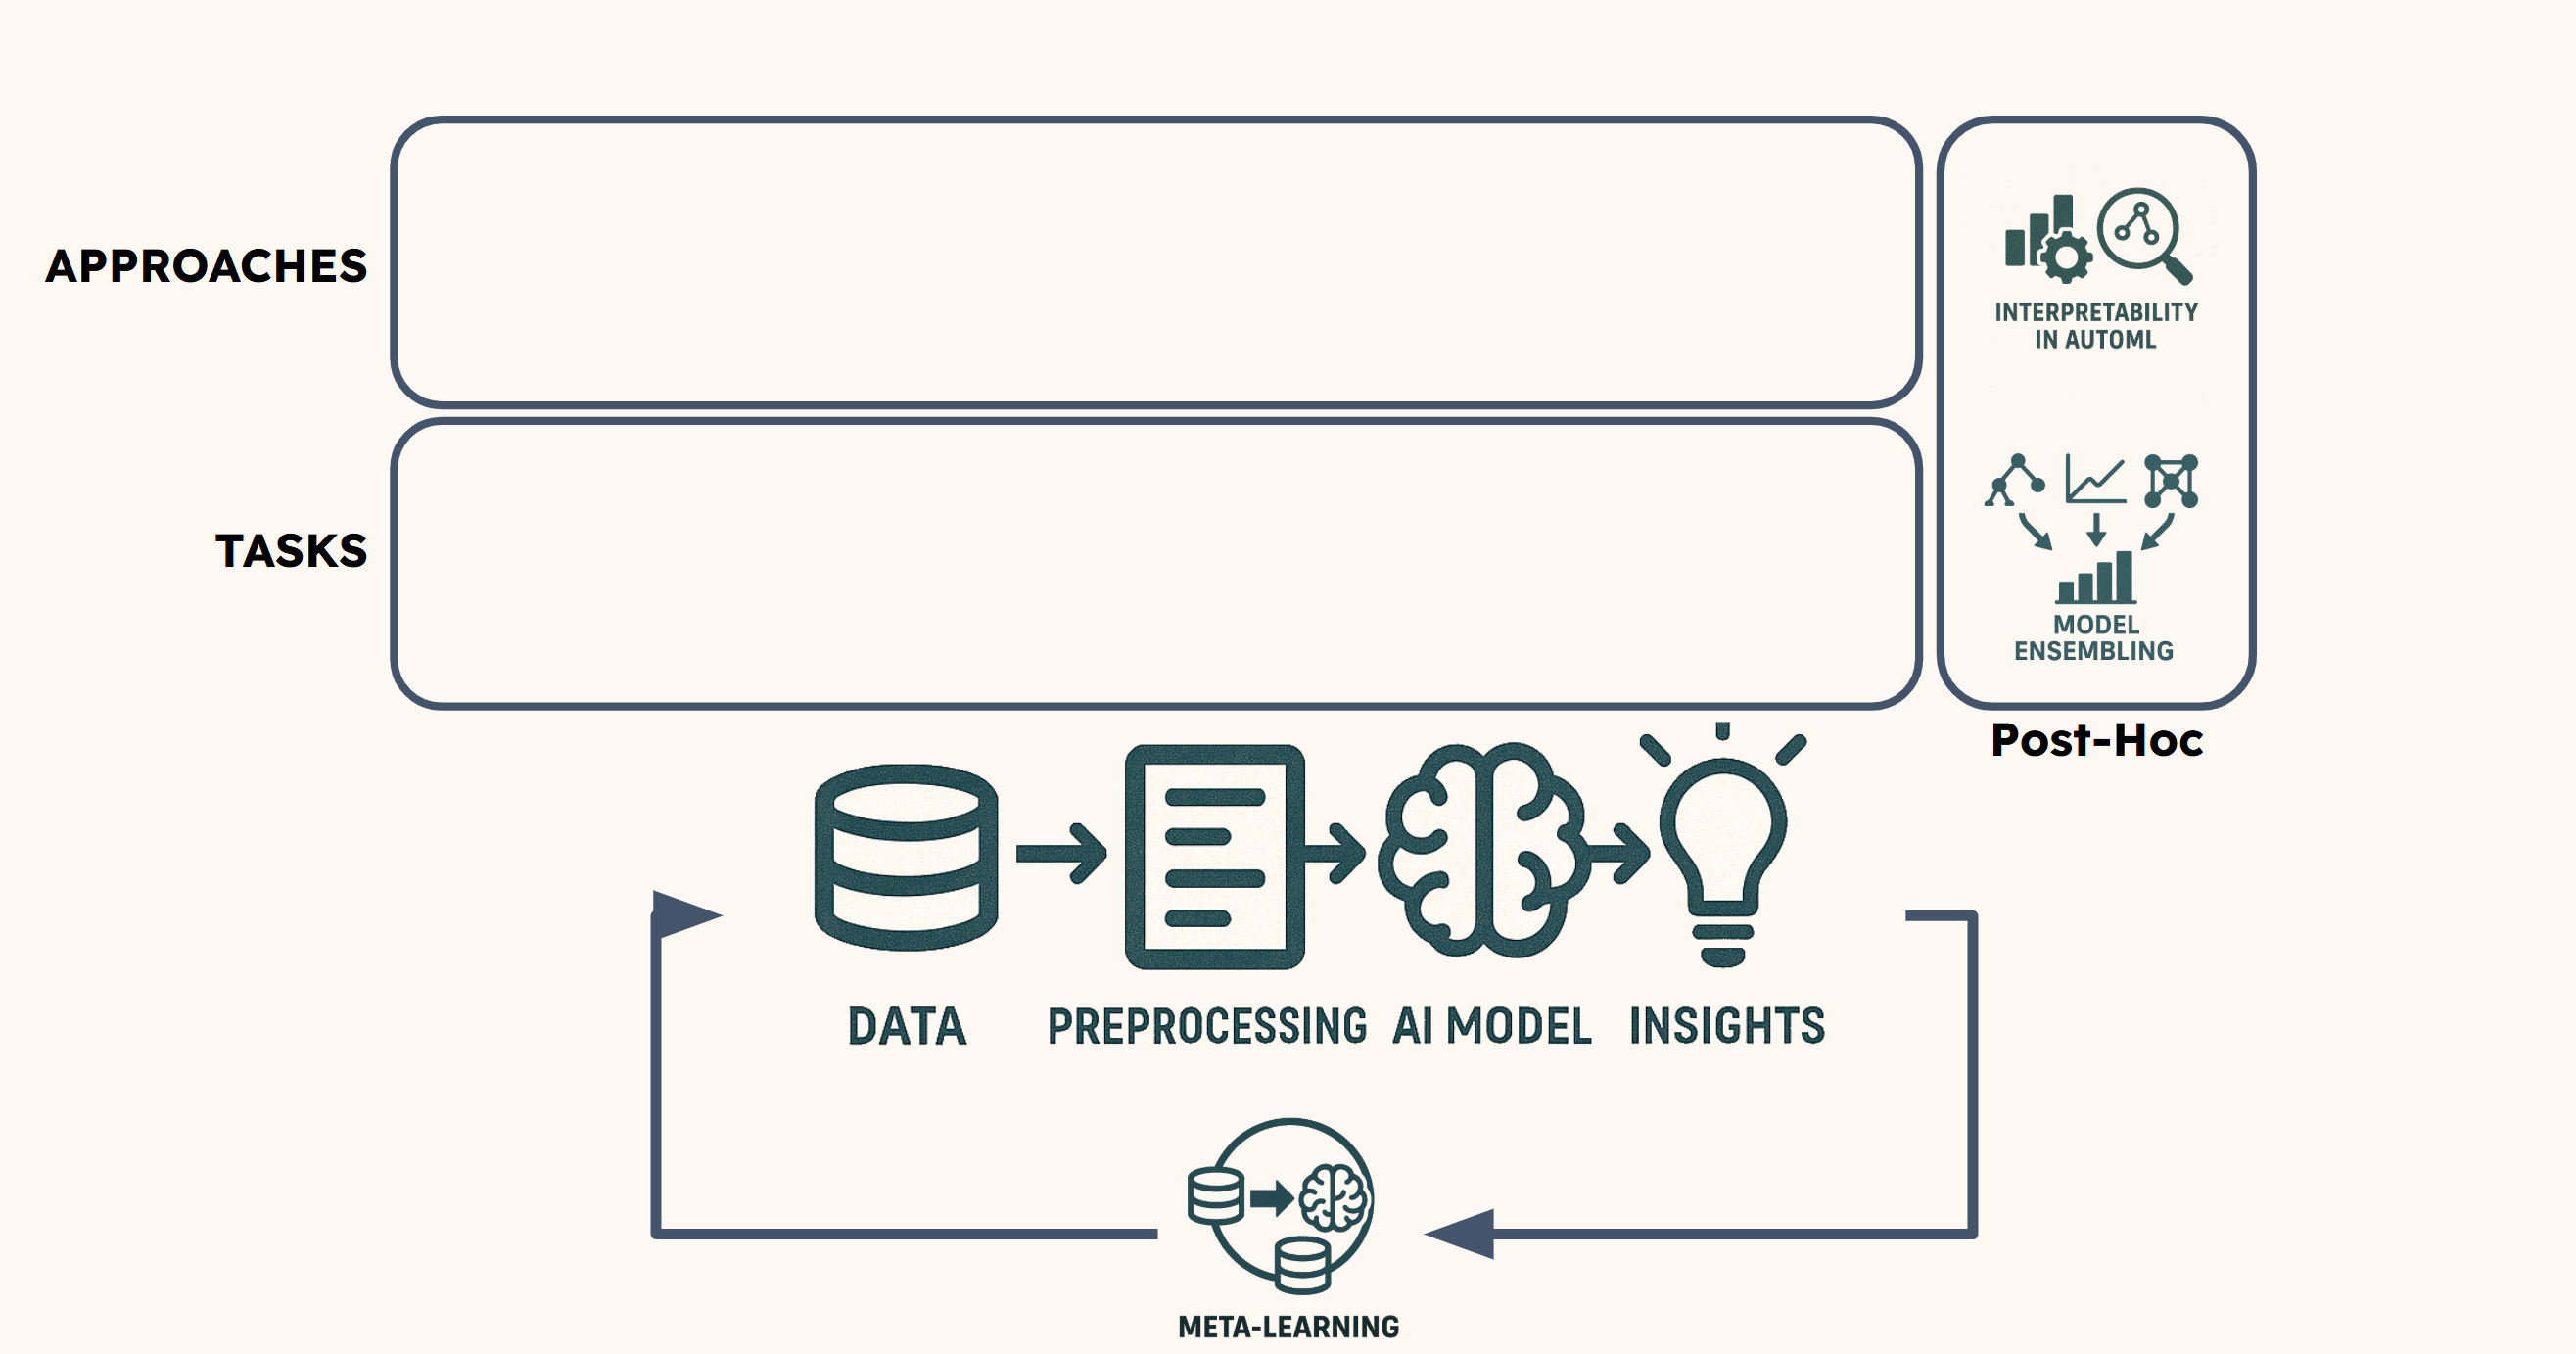
\includegraphics[width=0.8\textwidth]{images/automl_post-hoc.png}


\end{frame}
%-----------------------------------------------------------------------
%----------------------------------------------------------------------
\begin{frame}[c]{Overview AutoML Fields: Beyond}

\centering
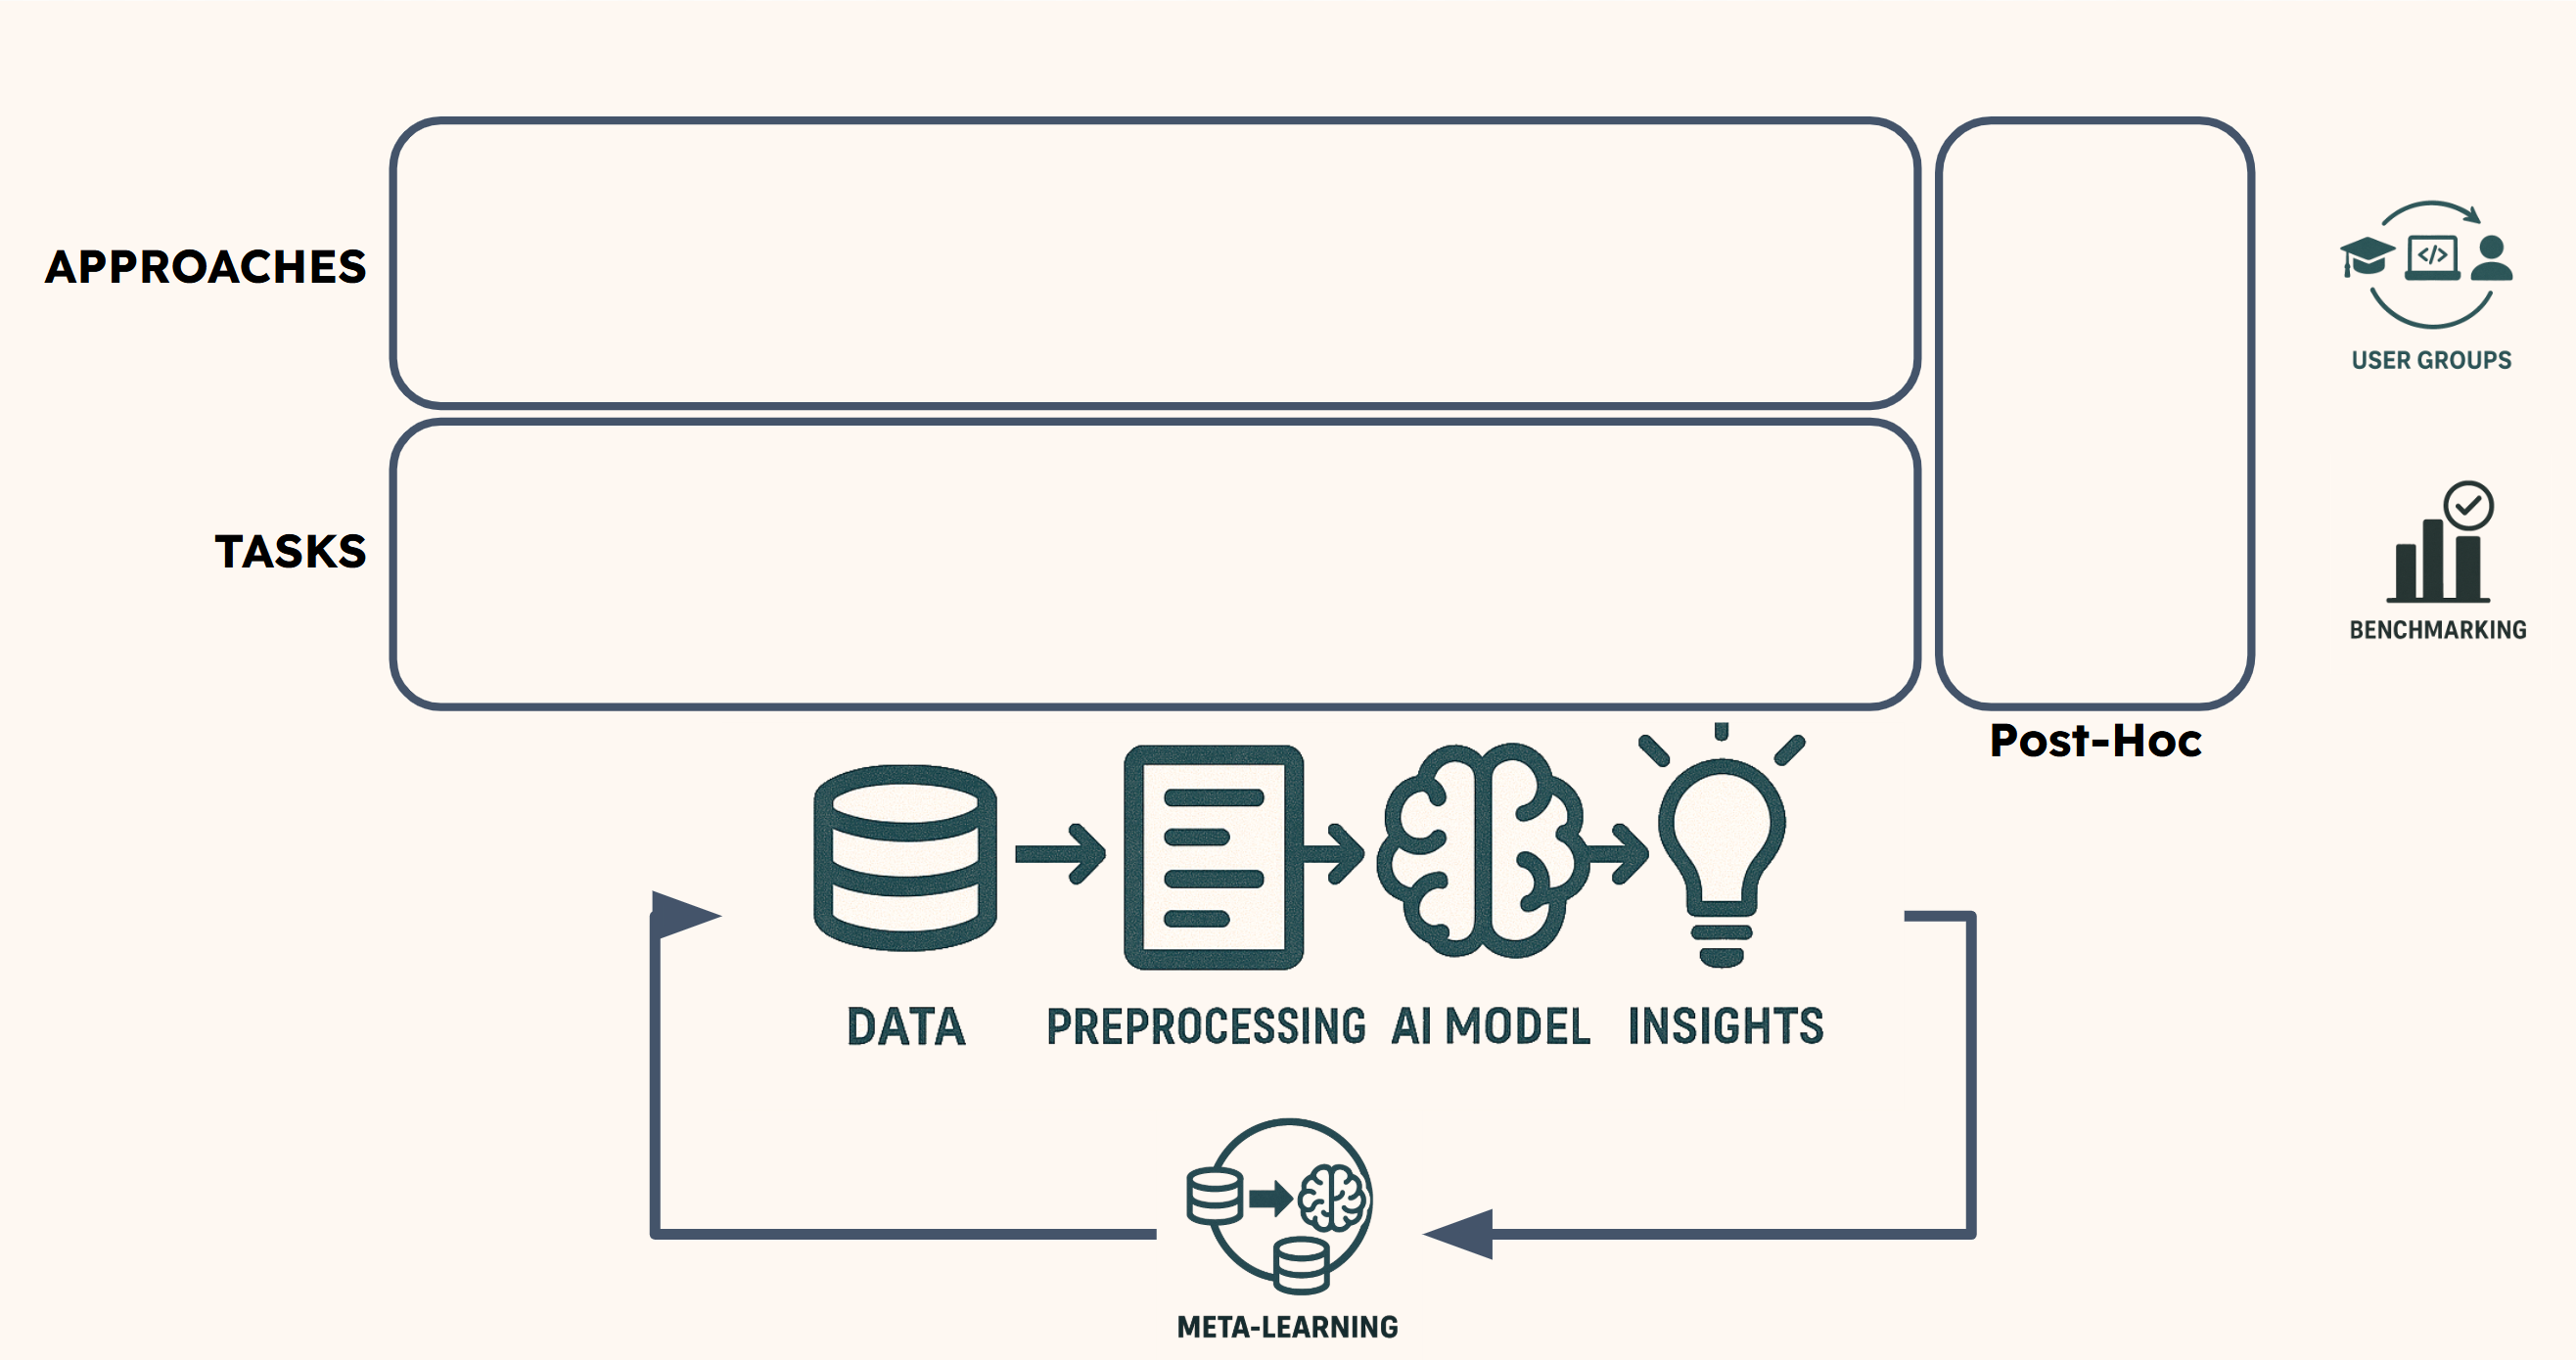
\includegraphics[width=0.8\textwidth]{images/automl_ext.png}


\end{frame}
%-----------------------------------------------------------------------
%----------------------------------------------------------------------
\begin{frame}[c]{Overview AutoML Fields: Full Picture}

\centering
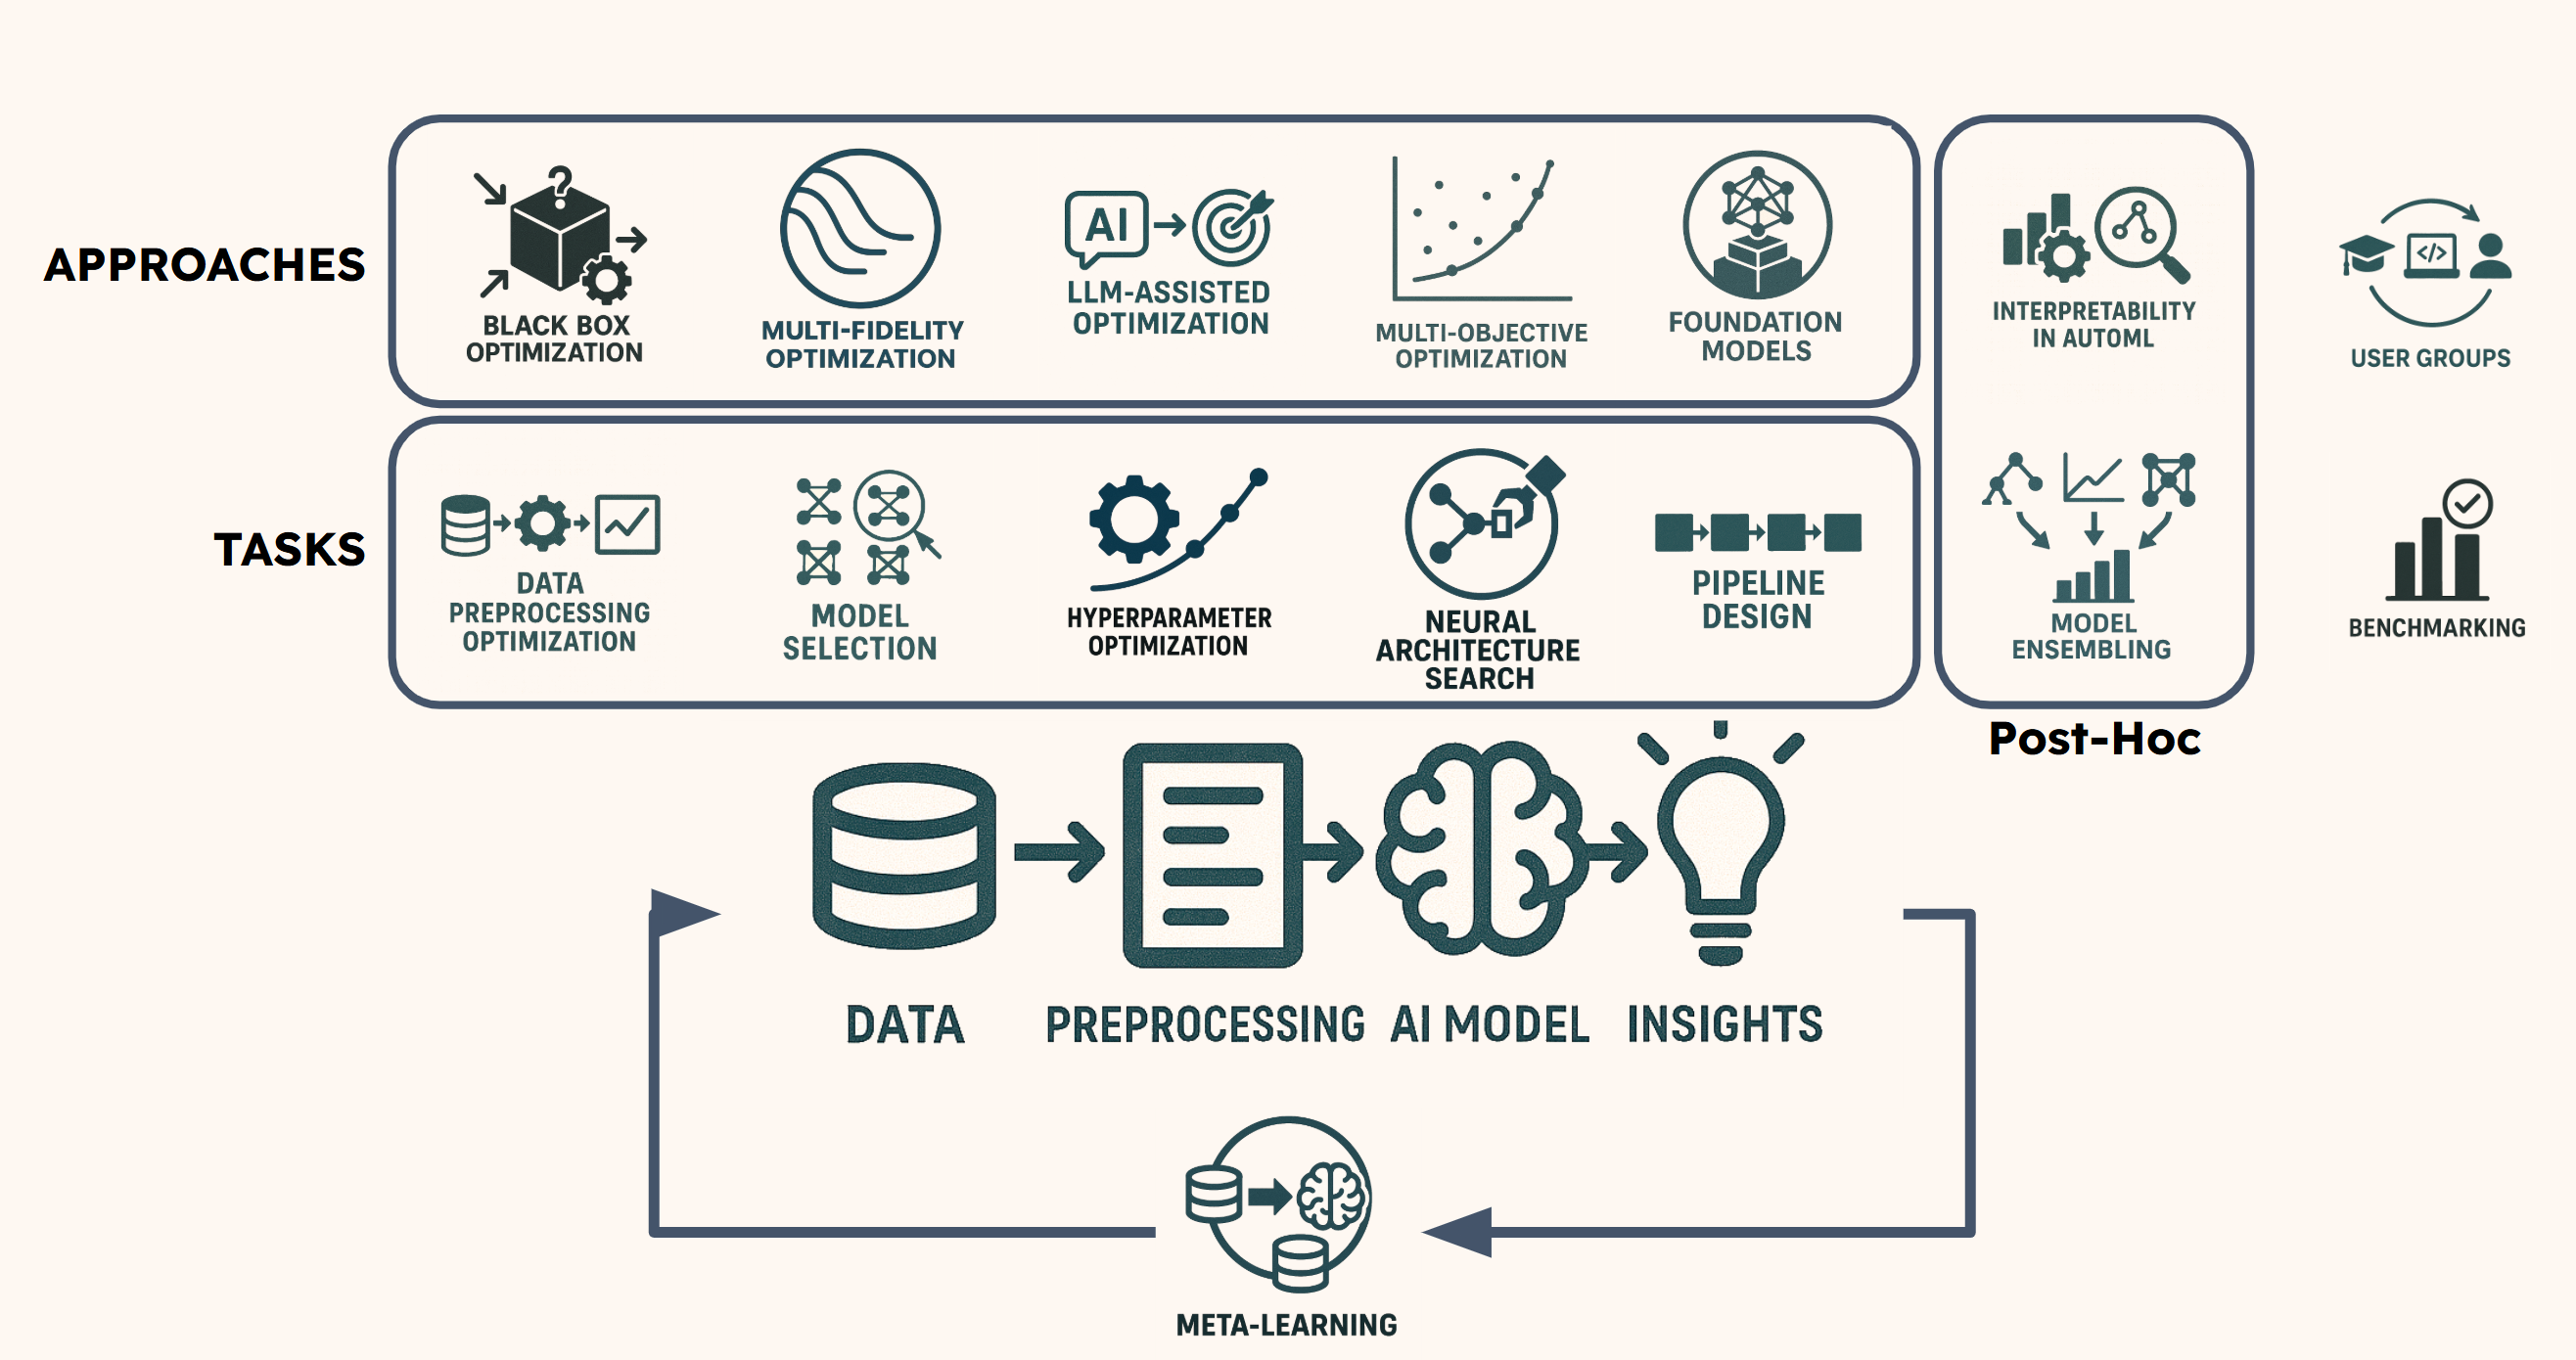
\includegraphics[width=0.8\textwidth]{images/automl_full.png}


\end{frame}
%-----------------------------------------------------------------------


%----------------------------------------------------------------------
\begin{frame}{Summary} 

Most important insights from this video:

\begin{enumerate}
    \item AutoML can be applied to the full pipeline design or individual tasks of the pipeline
    \item AutoML encompasses many different approaches for addressing the underlying problem
    \begin{itemize}
        \item There is no one-size-fits-all method
        \item Nevertheless, since we are on a meta-design level, there are diminishing returns in not choosing the best AutoML approach
    \end{itemize}
    \item AutoML leverages different techniques in post-processing (e.g., ensembling and stacking)
    \item Thinking about the users of AutoML and proper evaluations are crucial
\end{enumerate}


\end{frame}

\end{document}

